\documentclass[tikz, border=2pt]{standalone}
\usepackage{amsmath}

\begin{document}
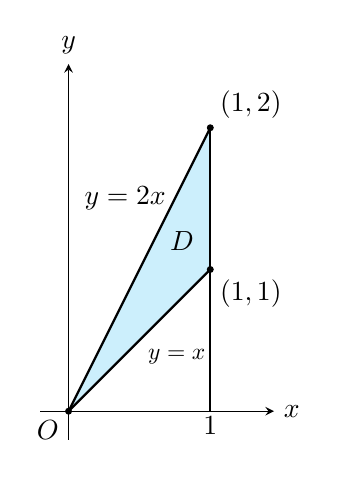
\begin{tikzpicture}[scale=1.8, >=stealth]
    \fill[cyan!20] (0,0) -- (1,1) -- (1,2) -- cycle;

    \draw[->] (-0.2, 0) -- (1.45, 0) node[right] {$x$};
    \draw[->] (0, -0.2) -- (0, 2.45) node[above] {$y$};

    \draw[thick] (0,0) -- (1,1) node[midway, below right, scale=0.85] {$y=x$};
    \draw[thick] (0,0) -- (1,2) ;
    \draw[thick] (1,0) -- (1,2) ;

    \fill (0,0) circle (0.7pt) node[below left] {$O$};
    \fill (1,1) circle (0.7pt) node[below right] {$(1,1)$};
    \fill (1,2) circle (0.7pt) node[above right] {$(1,2)$};

    \node at (0.8, 1.2) {$D$};
    \node at (0.4, 1.5) {$y=2x$};
    \node at (1,-0.1) {$1$};
\end{tikzpicture}
\end{document}
